\chapter{Entwurf}
\section{Genvorhersage}
\section{Das OSGi Framework}
%\begin{wrapfigure}{r}{9.0cm}
%	\begin{center}
%		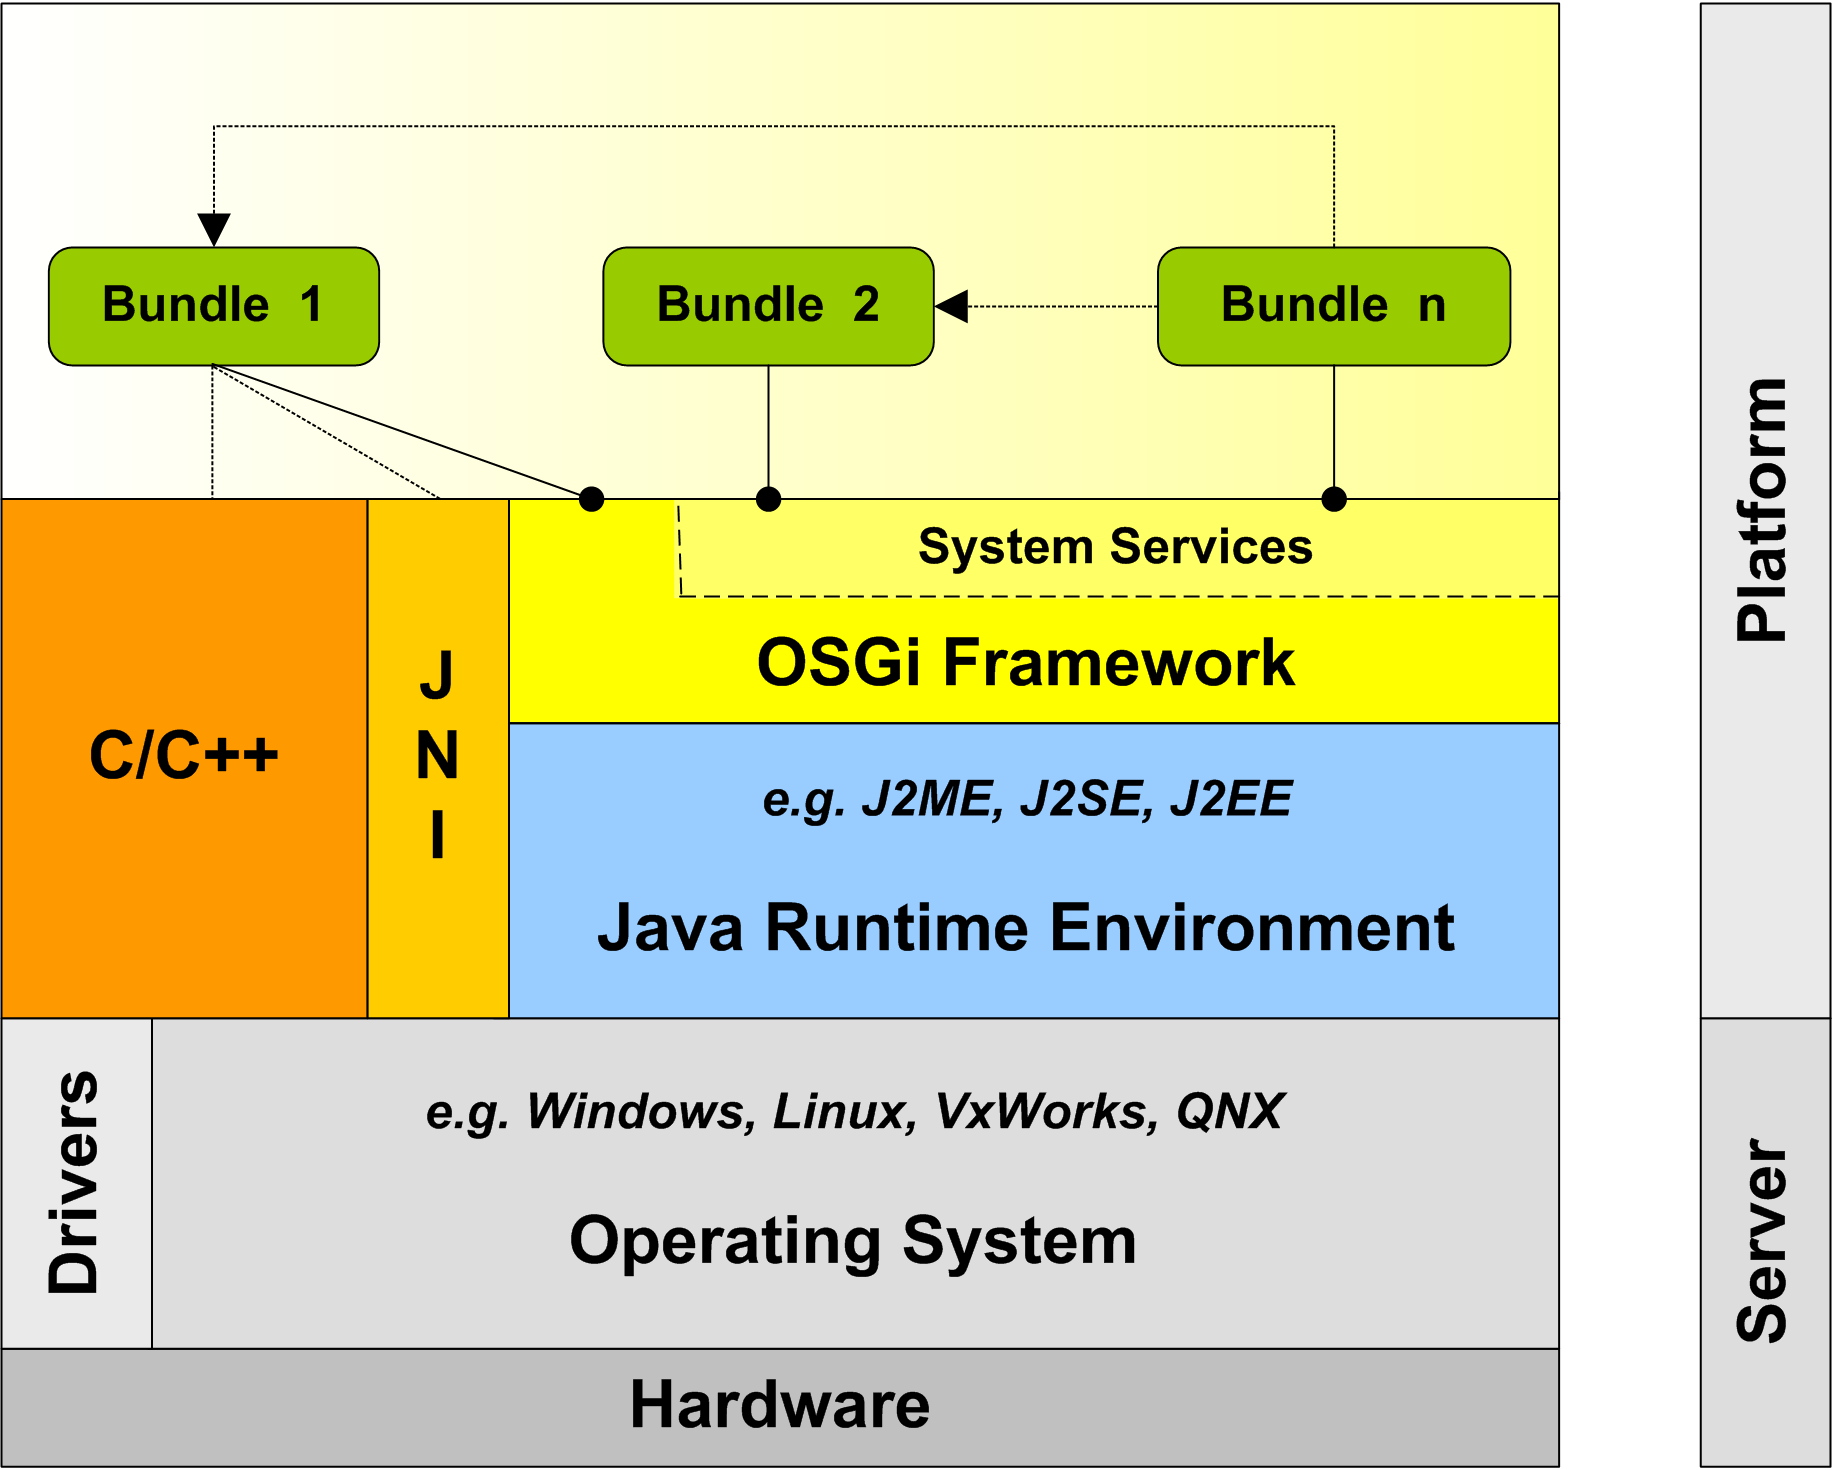
\includegraphics[width=8.5cm]{pics/osgi_layer.png}
%	\caption{something, citing}
%	\end{center}
%	\label{fig:hmm}
%\end{wrapfigure}
Die \textbf{OSGi Alliance}, früher
\enquote{\textit{Open Services Gateway initiative}}, ist ein Zusammenschluß
verschiedener Unternehmen, wie z.B. IBM, Oracle oder Sun Microsystems.
\index{OSGi Alliance}
\index{OSGi|see{OSGi Alliance}}
\index{Open Services Gateway|see{OSGi Alliance}}
Sie spezifiziert die \textbf{OSGi Service Platform}, ein Java-basiertes
Application-Framework, mit dessen Hilfe modulare, service-orientierte
Anwendungen erstellt werden können. Einzelne Module, sogenannte
\textbf{Bundles}, können der Anwendung dynamisch hinzugefügt und wieder
entfernt werden. Ein erneutes Kompilieren oder Starten der Anwendung ist dazu
nicht erforderlich.
\index{OSGi Service Platform}
\index{Bundle}
Das Framework bietet ausserdem eine globale \textbf{Service Registry}, an der
Bundles sogenannte \textbf{Services} anmelden und abgefragen können.
% OSGi Framework = OSGi Service Platform without OSGi Standard Services 13
\index{Service Registry}
\index{Service}
\begin{figure}[ht]
	\begin{center}
		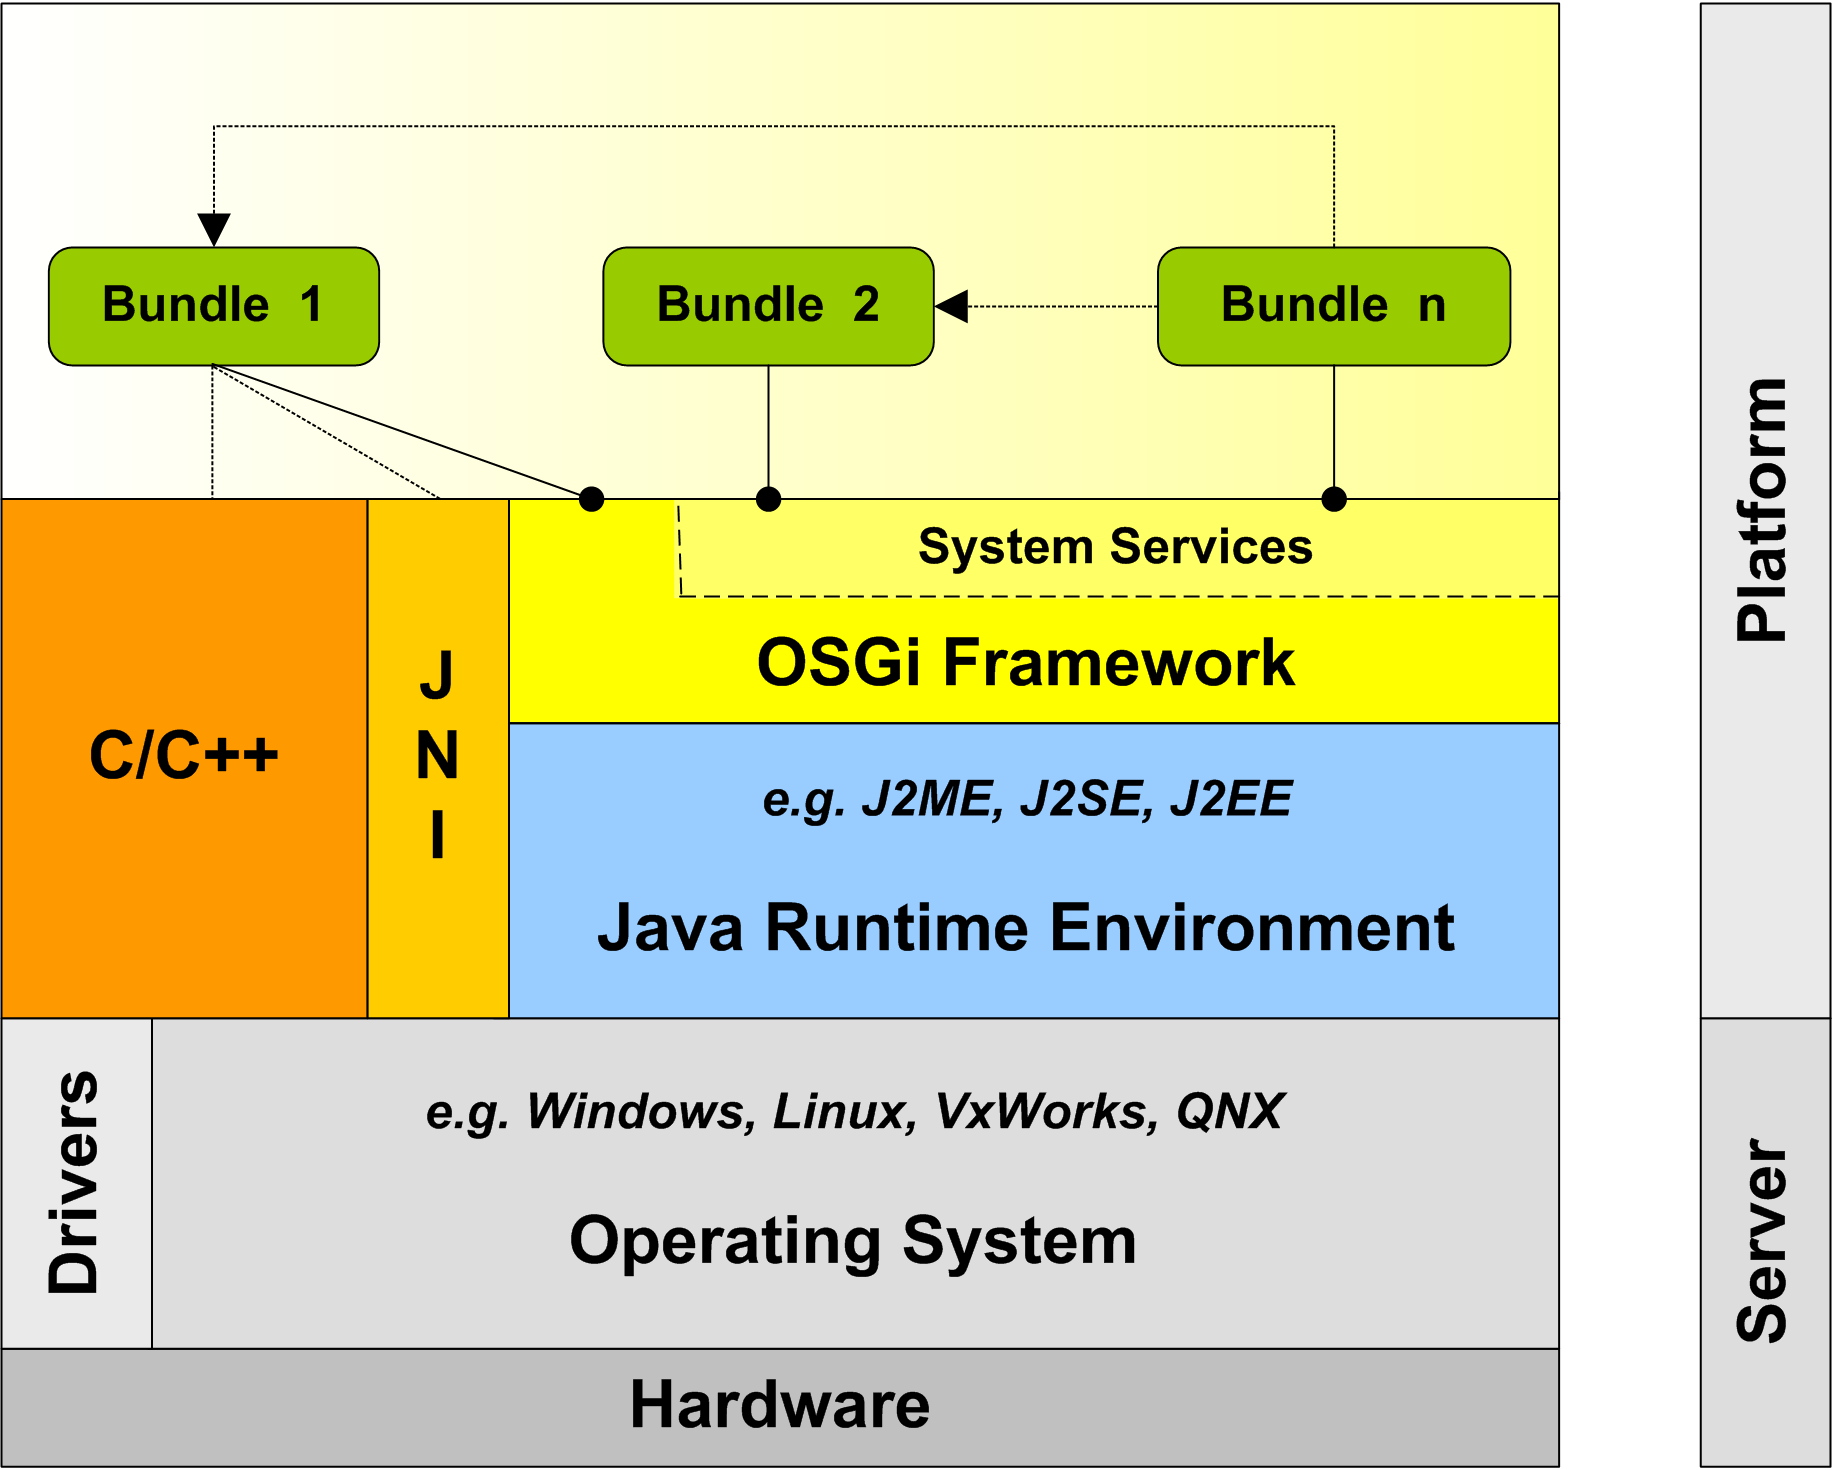
\includegraphics[scale=2]{pics/osgi_layer.png}
	\caption{something}
	\end{center}
	\label{fig:perfect}
\end{figure}
\subsection{Bundles}
Ein Bundle stellt technisch eine Einheit von Klassen und Ressourcen dar, die
eigentständig in der Anwenung gestartet, gestoppt, installiert und
deinstalliert werden können.
% selbe version 17
% importieren, exportieren 13 
% MANIFEST.MF 21
% lebenszyklen 23
% unterschied Bundle / Plug-In 41
\subsection{Services}
Ein Service ist ein Java-Object, typischerweise ein Interface, das unter dem
Interface-Namen an der Service Registry angemeldet wird.
\index{Service Registry}
Die Service Registry steht bundleübergreifend in der Anwendung zu Verfügung.
Wird ein bestimmer Dienst von einem Bundle benötigt, kann dieser an der Service
Registry abgefragt werden, ohne das im Enzelnen bekannt sein muss, welche
Implementierung dahinter steckt oder welches Bundle diesen Dienst anbietet.
% Services können kommen und gehen 23
% Standard Services 13,25
\citep{wtherich_die_2008}

